%
%   ATTENZIONARE INCERTEZZE NELLA TABELLA BETHE-BLOCH!! 4(5) VUOL DIRE \PM 5
%
\documentclass[oneside, a4paper, 11pt, final]{memoir}
\usepackage[T1]{fontenc}                % per il font
\usepackage[utf8]{inputenc}             % per l'input
\usepackage[english, italian]{babel}    % lingua principale inglese, secondaria italiano
%\input Rothdn.fd
%\newcommand*\initfamily{\usefont{U}{Rothdn}{xl}{n}}

\usepackage{layout}                 % per testare la formattazione del testo
\usepackage{lipsum}                 % anche lui per creare testo a caso
\usepackage{geometry}               % serve

\usepackage[intlimits]{amsmath}     % =======================================
\usepackage{amsfonts}               % cose utili per fare matematica e fisica
\usepackage{amssymb}                % intlimits mette gli estremi di integrazione sopra e sotto il segno di integrale       
\usepackage{amsthm}                 % cose utili per fare matematica e fisica
\usepackage{bbm}                    % cose utili per fare matematica e fisica
\usepackage{physics}                % cose utili per fare matematica e fisica
\usepackage{tensor}                 % =======================================
\usepackage{siunitx}
% \usepackage[scaled]{beramono}
\usepackage{inconsolata}

\usepackage{graphicx}               % per le foto
\usepackage{caption}                % per le caption
\usepackage{tikz}                   % per fare i disegnini belli
\usepackage{pgf}
\usepackage{pgfplots}
\usepackage{enumitem}               % 
\usepackage{listings}
\usepackage{emptypage}              % non se se serve
\usepackage{lettrine}               % per le lettere belle a inizio capitolo
% \usepackage{yfonts}                 % per le lettere belle a inizio capitolo

\usepackage{hyperref}               % fa le cross reference cliccabili dentro al testo (ad esempio da indice a capitolo)
                                    % ======================================

\usepackage{xurl}
\usepackage{csquotes}
\usepackage[backend = bibtex, style = numeric-comp, maxbibnames = 5]{biblatex}
  
\usepackage{misc/thesisutils}

% ---- REIMPOSTAZIONI ----
%=================%
%   PAGE LAYOUT   %
%=================%

\settypeblocksize{*}{1.2\lxvchars}{*}   % lxvchars è una dimensione raccomandata che dipende dal font, utile per la leggibilità
\setlrmargins{*}{*}{1}                  % setta i margini in modo che siano 1:1 adeguandosi al typeblock
\setulmarginsandblock{1.5in}{*}{1.4}    % setta i margini superiore e inferiore {superiore}{inferiore}{rapporto}
\checkandfixthelayout                   % does the magic

%=========================%
%   HEADER & PAGESTYLES   %
%=========================%

\setlength{\headwidth}{\textwidth}

\makepagestyle{thesis}                                                     % definisce il nome dello stile
\makerunningwidth{thesis}{\headwidth}                                      % definisce la lunghezza dell'header
\makeheadrule{thesis}{\headwidth}{\normalrulethickness}                    % mette la riga nell'header
\makeheadposition{thesis}{flushright}{flushleft}{flushright}{flushleft}    % definisce la posizione dell'header
\makepsmarks{thesis}{%                                                     % da qui in poi non lo so
    \nouppercaseheads
    \createmark{chapter}{both}{shownumber}{\chaptername\ }{.\ } 
    \createmark{section}{right}{shownumber}{}{.\ }              
    \createplainmark{toc}{both}{\contentsname}                  
    \createplainmark{lof}{both}{\listfigurename}                
    \createplainmark{lot}{both}{\listtablename}
    \createplainmark{bib}{both}{\bibname}
    \createplainmark{index}{both}{\indexname}
    \createplainmark{glossary}{both}{\glossaryname}    
}

%% se oneside:
    \makeoddhead{thesis}{\bfseries\leftmark}{}{\bfseries \thepage}
%% se twoside:
    % \makeevenhead{thesis}{\bfseries\thepage}{}{\bfseries\leftmark}
    % \makeoddhead{thesis}{\bfseries\rightmark}{}{\bfseries

\chapterstyle{hangnum}
\aliaspagestyle{chapter}{empty}                                             % toglie il numero di pagina nelle pagine con il nome del capitolo.
\newcommand{\initcolor}{purple}

%===============%
%   NUMBERING   %
%===============%

\numberwithin{equation}{chapter}    % Aggiunge il numero del capitolo all'equazione
\setsecnumdepth{subsection}         % numera le subsection (1.1.1)

\hypersetup{                    % ======================================
    colorlinks=true,            % template preso da internet
    linkcolor=black,            % molto sobrio, le cose cliccabili si evidenziano quando passi il mouse
    filecolor=black,            %
    urlcolor=blue,              %
    pdfpagemode=FullScreen,     %
    citecolor=black,            %
}

\definecolor{codegreen}{rgb}{0,0.6,0}
\definecolor{codegray}{rgb}{0.5,0.5,0.5}
\definecolor{codepurple}{rgb}{0.58,0,0.82}
\definecolor{codeorange}{rgb}{0.5,0.5,0}
\definecolor{backcolour}{rgb}{0.97,0.98,0.98}

\lstdefinestyle{mystyle}{
    backgroundcolor=\color{backcolour},   
    commentstyle=\color{codegreen},
    keywordstyle=\color{magenta},
    numberstyle=\tiny\color{codegray},
    stringstyle=\color{codepurple},
    %variablestyle=\color{codeorange},
    basicstyle=\ttfamily\footnotesize,
    breakatwhitespace=false,         
    breaklines=true,
    breakindent=0pt,                 
    captionpos=b,                    
    keepspaces=true,                 
    numbers=left,
    frame=tblr,
    rulecolor=\color{black},
    numbersep=5pt,                  
    showspaces=false,                
    showstringspaces=false,
    showtabs=false,                  
    tabsize=4,
    columns=fixed,
}

\lstset{style=mystyle}

\begin{document}
    % \newgeometry{margin=70pt}
% \begin{titlingpage}
%     \begin{center}
%         \begin{minipage}[b]{0.5\textwidth}
%             \flushleft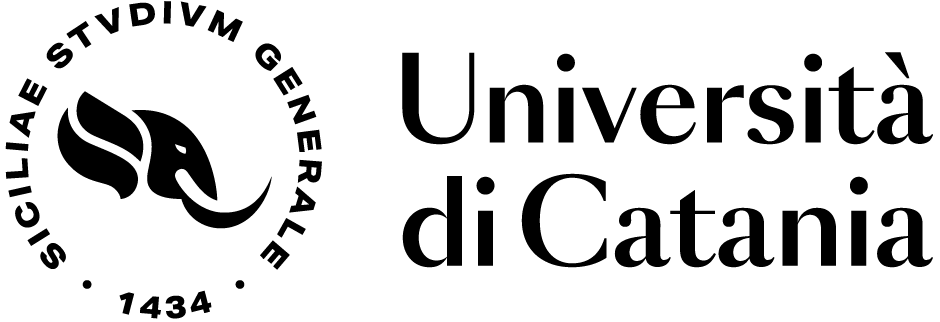
\includegraphics[height = 70pt]{images/UniCT-Logo-Nero1.png}
%         \end{minipage}
%         \hspace{\fill}
%         \begin{minipage}[b]{0.45\textwidth}
%             \flushright
\includegraphics[height = 70pt]{images/LogoDFA.png}
%         \end{minipage}%
%         \\[10pt]
%         \hrule\vspace{5pt}\hrule
%         \vspace{\fill}
%         \textbf{\huge{TESINA}}
%         \vspace{\fill}\
%         \vspace{\fill}
%         \hrule
%         \vspace{5pt}
%         \textbf{Anno Accademico 2024--2025}
%     \end{center}
% \end{titlingpage}
% \restoregeometry

\newgeometry{margin=1in}
\newcommand{\unictsize}{0.3\textwidth}
\newcommand{\dfasize}{0.6\textwidth}
\newcommand{\namesize}{0.8\textwidth}
\newcommand{\doublerule}{\hrule \vspace{5pt} \hrule}

\begin{titlingpage}
    \begin{center}
        \begin{minipage}[h!]{\linewidth}
            \begin{minipage}[ht!]{\linewidth}
                \centering
                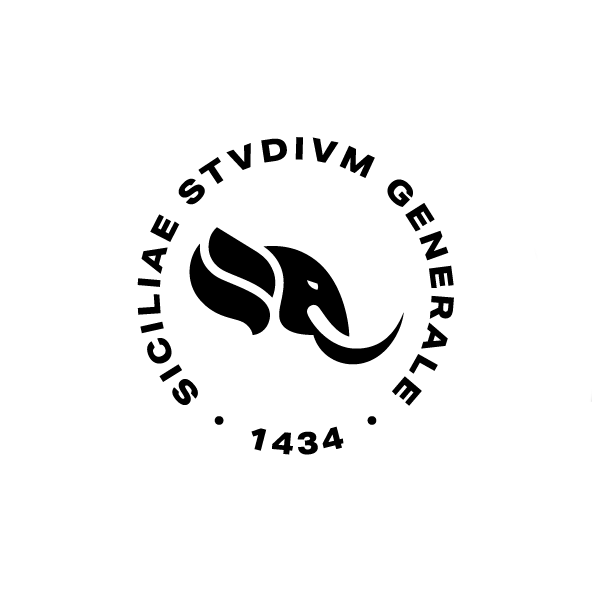
\includegraphics[width=\unictsize]{images/UniCT-Logo-Nero-quadrato.png}
            \end{minipage}
            \centering\large
            \textbf{UNIVERSITÀ DEGLI STUDI DI CATANIA}
            \\[5pt]
            \normalsize
            \textsc{Dipartimento di Fisica e Astronomia ``Ettore Majorana''}
            \\[5pt]
            \textsc{Corso di Laurea in Fisica}
            \\[10pt]
            \doublerule
        \end{minipage}
        \\[50pt]
        \vspace{\fill}
        {\huge\bfseries Relazioni di\\Laboratorio di Fisica 3\\}
        % \begin{tikzpicture}
        %     \draw (0, 0) node[inner sep=0,nearly transparent] {\includegraphics[width=\dfasize]{images/dfa-logo.png}};
        %     \draw (0, 1) node {\huge{\textbf{METODI SIMPLETTICI}}};
        %     \draw (0, 0) node {\huge{\textbf{PER LE EQUAZIONI}}};
        %     \draw (0, -1) node {\huge{\textbf{DI EINSTEIN}}};
        % \end{tikzpicture}
        %\huge{\textbf{TITOLO\\\vspace{5pt}DELLA TESI}}\normalsize
        \vfill
        \centering
        \begin{minipage}[h]{\unictsize}
            \centering
            \hrule
            \vspace{10pt}
            \textsc{Le quattro cose}
            \vspace{10pt}
            \hrule
        \end{minipage}
        \\[50pt]
        \vspace{\fill}
        \vspace{30pt}
        \doublerule
        \vspace{10pt}
        \normalsize
        \textbf{Anno Accademico 2024 -- 2025}
    \end{center}
\end{titlingpage}
\restoregeometry
    \pagestyle{thesis}

    \frontmatter
        \tableofcontents
        \chapter{Sommario}
    \lettrine[loversize=0.08, lines=2]{I}{n questo} documento sono raccolte le quattro relazioni brevi da svolgere durante il corso annuale di \emph{Laboratorio di Fisica 3} del Corso di Laurea in \emph{Fisica} presso l'Università degli Studi di Catania.

    Le quattro espserienze sono esposte nei quattro capitoli seguenti. 

    \mainmatter
        \chapter[Implementazione Numerica della Formula di Bethe--Bloch][Formula di Bethe--Bloch]{Implementazione Numerica della Formula di Bethe--Bloch}\label{ch:bet}

\section{Il modello}
    Come descritto dal Particle Data Group \cite{PhysRevD-110-030001}, la formula di Bethe--Bloch è un modello sperimentale che descrive la perdita di energia di particelle cariche pesanti di media energia---come protoni e particelle $\alpha$---nella materia:
    \begin{equation}
        \left\langle -\dv{E}{x}\right\rangle
        = Kz^2 \frac{Z}{A}\frac{1}{\beta^2}\bqty{\frac{1}{2}\log\frac{2 m_e c^2 \beta^2 \gamma^2 W_\text{max}}{I^2} - \beta^2 - \frac{\delta\pqty{\beta\gamma}}{2}}
        \mycomma
        \label{eq:bet:bethe-bloch-1}
    \end{equation}
    dove $\beta$ e $\gamma$ sono le usuali quantità relativistiche mentre il resto dei simboli sono esplicitati in \tabref{tab:bet:costanti}.
    \begin{table}
        \footnotesize
        \centering
        \begin{tabular*}{\textwidth}{@{\extracolsep{\fill}}lll}\hline\rule{0pt}{8pt}%
    Simbolo & Definizione & Valore o unità di misura\\[0.5pt]
    \hline\hline\rule{0pt}{9pt}%
    $m_e c^2$ & massa a riposo dell'elettrone $\times c^2$ & \SI{ 0.51099895000(15)}{\mega\eV}\\
    $r_e$ & raggio classico dell'elettrone $ e^2/4\pi \epsilon_0 m_e c^2$ & \SI{2.8179403227(19)}{\femto\meter}\\
    $N_\text{A}$ & numero di Avogadro & \SI{ 6.022140857(74)e+23}{mol^{-1}}\\[2pt]
    \hline\rule{0pt}{9pt}%
    $\rho$ & densità & \unit{\g\,\centi\meter^{-3}}\\
    $x$ & massa per unità di area & \unit{\gram\,\centi\meter^{-2}}\\ 
    $M$ & massa della particella incidente & \unit{\mega\eV \,\mathit{c}^{-2}}\\
    $E$ & energia della particella incidente $\gamma M c^2$ & \unit{\mega\eV}\\
    $W_\text{max}$ & massima energia trasferibile per collisioni & \unit{\mega\eV}\\
    $z$ & numero di carica della particella incidente & \\
    $Z$ & numreo atomico del bersaglio & \\
    $A$ & numero di massa atomica del bersaglio & \\
    $K$ & $4\pi N_\text{A} r_e^2 m_e c^2$ & \SI{0.307075}{\mega\eV\,\mol^{-1}\,\centi\meter^2}\\
    $I$ & energia media di eccitazione & \unit{\eV}\\
    $\delta\pqty{\beta\gamma}$ & correzione di ionizzazione & \\[1pt]
    \hline
\end{tabular*}
        \caption{Notazione e unità di misura per la formula di Bethe--Bloch. Si tratta di un riassunto della tabella del PDG \cite{PhysRevD-110-030001}.}
        \label{tab:bet:costanti}
    \end{table}
    La perdita di energia media data dalla \eqref{eq:bet:bethe-bloch-1} è misuarta in \unit{\mega\eV\,\gram^{-1}\,\centi\meter^2} ma può essere portata in \unit{\mega\eV\,\centi\meter^{-1}} moltiplicando entrambi i membri per la densità volumica $\rho$ del bersaglio misurata in \unit{\gram\,\centi\meter^{-3}}. La quantità $W_\text{max}$ è la massima energia che una particella carica può cedere a un elettrone e si esprime come
    \begin{equation}
        W_\text{max} = \frac{2 m_e c^2 \beta^2 \gamma^2}{1 + \gamma\, m_e / M + (m_e / M)^2}
        \myperiod 
        \label{eq:bet:wmax}
    \end{equation}
    La \eqref{eq:bet:bethe-bloch-1} e la \eqref{eq:bet:wmax} sono valide nell'approssimazione $\num{0.1} \lesssim \beta\gamma \lesssim \num{1000}$ poiché al limite inferiore la velocità del proiettile diventa confrontabile con la ``velocità'' degli elettroni atomici mentre al limite superiore gli effetti radiativi non sono più trascurabili.

\section{La simulazione}
    Ho scelto di simulare la perdita di energia di una particella $\alpha$ a \SI{5}{\mega\eV} attraverso un foglio di alluminio di spessore\footnote{Dopo aver provato con uno spessore di \SI{0.016}{\milli\meter} e aver constatato che la curva risultava tagliata---la particella non cedeva tutta l'energia all'alluminio---ho scelto di aumentare di poco lo spessore per il gusto di un grafico più completo.} \SI{0.018}{\milli\meter}. Per realizzare la simulazione ho scritto un codice in C che implementa la \eqref{eq:bet:bethe-bloch-1} in modo approssimato.
    \subsection{Descrizione del codice e dei calcoli}
        Il programma inizia richiedendo da tastiera il numero di intervalli $N$ in cui suddividere lo spessore del materiale; gli altri dati sono tutti precompilati come costanti. 
        
        Assumiamo che in ciascun intervallo di spessore\footnote{Ricordo che in questo caso la $x$ non indica una distanza.} $\dd{s}$ tutte le quantità variabili di nostro interesse siano costanti---velocità, energia, perdita di energia \myetc. Dalla teoria della relatività ristretta scriviamo per l'$n$-esimo intervallo
        \begin{align*}   
                E_n &= T_n + M c^2 \mycomma \\
                E_n &= \gamma_n M c^2 \mycomma
        \end{align*}
        dove $M$ è la massa a riposo della particella incidente, $T_n$ la sua energia cinetica ed $E_n$ la sua energia totale. Note queste ultime due quantità, è possibile calcolare il fattore di Lorentz $\gamma_n$ e $\beta_n^2$ come
        \begin{equation*}
            \gamma_n = \frac{T_n + M c^2}{M c^2}
            \,,
            \quad
            \beta_n^2 = 1 - \frac{1}{\gamma_n^2}
            \myperiod
        \end{equation*}
        Le quantità appena descritte sono calcolate attraverso il codice nelle righe \lnref{ln:bet:T-start}--\lnref{ln:bet:T-end}.

        Noti $\gamma_n$ e $\beta_n$, è possibile calcolare la perdita di energia media per unità di lunghezza attraverso la \eqref{eq:bet:bethe-bloch-1} moltiplicata per $\rho$. Possiamo in particolare calcolare l'energia cinetica con cui la particella $\alpha$ entra nello strato successivo, $T_{n + 1}$ come
        \begin{equation*}
            T_{n + 1} = T_n + \dd{T_n} = T_n + \rho\, {\left\langle - \dv{E}{x} \right\rangle}_n \dd{s}
            \mycomma
        \end{equation*}
        essendo naturalmente $\dd{T_n} \leq 0$. Il calcolo di $\rho\,\abs{{\left\langle - \dd{E} / \dd{x} \right\rangle}_n}$ è svolto dalla funzione \texttt{bethe()} chiamata alla riga \lnref{ln:bet:bethe-call} e definita alla riga \lnref{ln:bet:bethe-def}, con l'ausilio della funzione \texttt{wmax()} che in particolare calcola il termine $W_\text{max}$.

        Il calcolo viene quindi ripetuto a partire dalla nuova energia $T_{n + 1}$ per ottenere la perdita di energia attraverso il successivo strato. Per ogni reiterazione il codice stampa su un file la distanza totale percorsa, l'energia cinetica della particella e la quantità $\abs{\dd{T_n}} = \rho\,\abs{{\left\langle - \dd{E} / \dd{x} \right\rangle}_n}$.

    \subsection{Risultati della simulazione}
        \begin{figure}
            \centering
            \begin{tikzpicture}
    \begin{axis}[
        width   = \plotsize,
        height  = 0.6\plotsize,
        xlabel  = {Distanza (\unit{\centi\meter})},
        ylabel  = {Energia $\alpha$ (\unit{\mega\eV})},
        xmin    = 0.0000,   xmax = 0.0022,  xtick = {0.0000,0.0002,...,0.0022},
        ymin    = 0.0,      ymax = 5.0,     ytick = {0.0,1.0,...,5.0},
        tick align = outside,
    ]
        \addplot+ [
            only marks,
            mark        = *,
            mark size   = 0.5pt,
            draw        = black,
            fill        = black,
        ] table [
            x index = 0,
            y index = 1,
            col sep = space
        ] {data/bethebloch/better-data.dat};
    \end{axis}
\end{tikzpicture}
            \begin{tikzpicture}
    \begin{axis}[
        width   = \plotsize,
        height  = 0.6\plotsize,
        xlabel  = {Distanza (\unit{\centi\meter})},
        ylabel  = {$\rho\abs{\left\langle - \dd{E} / \dd{x} \right\rangle}$  (\unit{\mega\eV\,\centi\meter^{-1}})},
        xmin    = 0.0000,   xmax = 0.0022,  xtick = {0.0000,0.0002,...,0.0022},
        ymin    = 0.00,     ymax = 4000,    ytick = {0.0,500,...,4000},
        tick align = outside,
    ]
        \addplot+ [
            only marks,
            mark        = *,
            mark size   = 0.5pt,
            draw        = black,
            fill        = black,
        ] table [
            x index = 0,
            y index = 2,
            col sep = space
        ] {data/bethebloch/better-data.dat};
    \end{axis}
\end{tikzpicture}
            \caption{In alto l'energia della particella $\alpha$ che diminuisce man mano che la particella penetra l'alluminio. In basso il potere d'arresto con l'evidente picco di Bragg.}
            \label{fig:bet:alpha}
        \end{figure}
        Osserviamo adesso i dati che si ottengono inserendo nel programma un numero arbitrariamente alto di step pari a \num{500}. In \figref{fig:bet:alpha} sono riportati in due grafici i valori dell'energia cinetica della particella $\alpha$ e del potere d'arresto del materiale al variare della distanza percorsa.
        
        Dal primo grafico risulta evidente la decrescita dell'energia della particella. Si nota che l'energia cinetica non si annulla del tutto, nonostante si avvicini ragionevolmente a \SI{0}{\mega\eV}: questo può essere dovuto a imprecisioni nel codice come il modo in cui vengono gestiti valori di $T$ negativi e valori di $\dd{T}$ che farebbero aumentare l'energia.

        Nel secondo grafico invece è riportato l'andamento del potere d'arresto, detto comunemente \emph{curva di Bragg}. L'energia depositata dalla particella $\alpha$ è inversamente proporzionale al quadrato della velocità, per questo subito prima del totale arresto si osserva il massimo deposito di energia nel tratto di grafico detto \emph{picco di Bragg}.
        \newcommand{\tmp}{TMP36}
\newcommand{\vs}{\texttt{+vs}}
\newcommand{\vout}{\texttt{vout}}
\newcommand{\gnd}{\texttt{gnd}}
\newcommand{\pinV}{\texttt{5v}}
\newcommand{\sensorpin}{\texttt{A0}}
\newcommand{\txtloop}{\texttt{loop}}

\chapter{Misura di Temperature con Arduino}
    Tra le esperienze svolte con Arduino Uno riporto in particolare la misura della variazione della temperatura della mia stanza da letto in seguito all'accensione del riscaldamento in casa.

    \section{L'esperimento}
            L'obiettivo dell'esperienza è quello di valutare qualitativamente l'andamento della temperatura della stanza per fare una stima di quanto velocemente si riscaldi e a quale temperatura tenda asintoticamente.

        \subsection{Preparazione della stanza}\label{ss:ard:preparazione}
            Per massimizzare l'escursione termica ho effettuato la misura durante una sera invernale avendo preventivamente aperto le finestre per abbassare la temperatura della stanza.
            
            Per migliorare la circolazione dell'aria ed evitare un eccessivo gradiente di temperatura---il radiatore caldo si trova in un angolo della stanza mentre i vetri freddi della finestra si trovano dal lato opposto---ho acceso dei ventilatori: uno a soffitto per limitare la raccolta dell'aria calda in alto e un più piccolo ventilatore da tavolo per allontanare l'aria calda dal radiatore e facilitare il riscaldamento dell'aria fredda.
            
            Infine, per isolare il più possbile il sistema, ho chiuso le tende sulla finestra per ridurre la dispersione di calore attraverso il vetro freddo e mantenuto la porta chiusa per non disperdere calore nel resto della casa.

        \subsection{Strumenti utilizzati}
            Gli strumenti utillizzati per la presa dei dati sono:
            \begin{enumerate}[label=$\bullet$]
                \item Una microcontrollore Arduino Uno con un sensore di temperatura \tmp;
                \item Un computer per compilare ed eseguire il codice sulla scheda Arduino e prelevare i dati.
            \end{enumerate}

            Il sensore \tmp\ è un sensore di temperatura a semiconduttore pensato per operare in un range di temperature che va da \SI{-40}{\celsius} a $+\SI{125}{\celsius}$. Esso presenta tre pin: \vs, \vout\ e \gnd. Il primo e l'ultimo servono per l'alimentazione che deve essere compresa tra \SI{2.7}{\volt} e \SI{5.5}{\volt} con una corrente inferiore ai \SI{50}{\micro\ampere}, che garantisce un surriscaldamento per effetto Joule trascurabile. Il secondo pin invece sestituisce una differenza di potenziale rispetto al \gnd\ proporzionale alla temperatura misurata. La sensibilità del sensore fornita dal costruttore è di \SI{\pm 1}{\celsius} e il suo fattore di scala è di \SI{10}{\milli\volt\per\celsius}  \cite{tmp36-datasheet}.

            La scheda Arduino attraverso i pin analogici accetta in input delle differenze di potenziale che vanno da \SI{0}{V} a \SI{5}{V} che vengono convertite in un segnale digitale che assume valori discreti da \num{0} a \num{1023}.

        \subsection{Circuito e codice}\label{ard:codice}
            Il circuito realizzato per l'esperimento è quello rappresentato in \figref{fig:arduino-1}. L'alimentazione al sensore è fornita tramite i pin \pinV\ e \gnd\ mentre il segnale in uscita dal sensore viene letto dal pin \sensorpin\ della scheda.

            \begin{figure}[t]
                \centering
                    \begin{minipage}{0.49\textwidth}
                        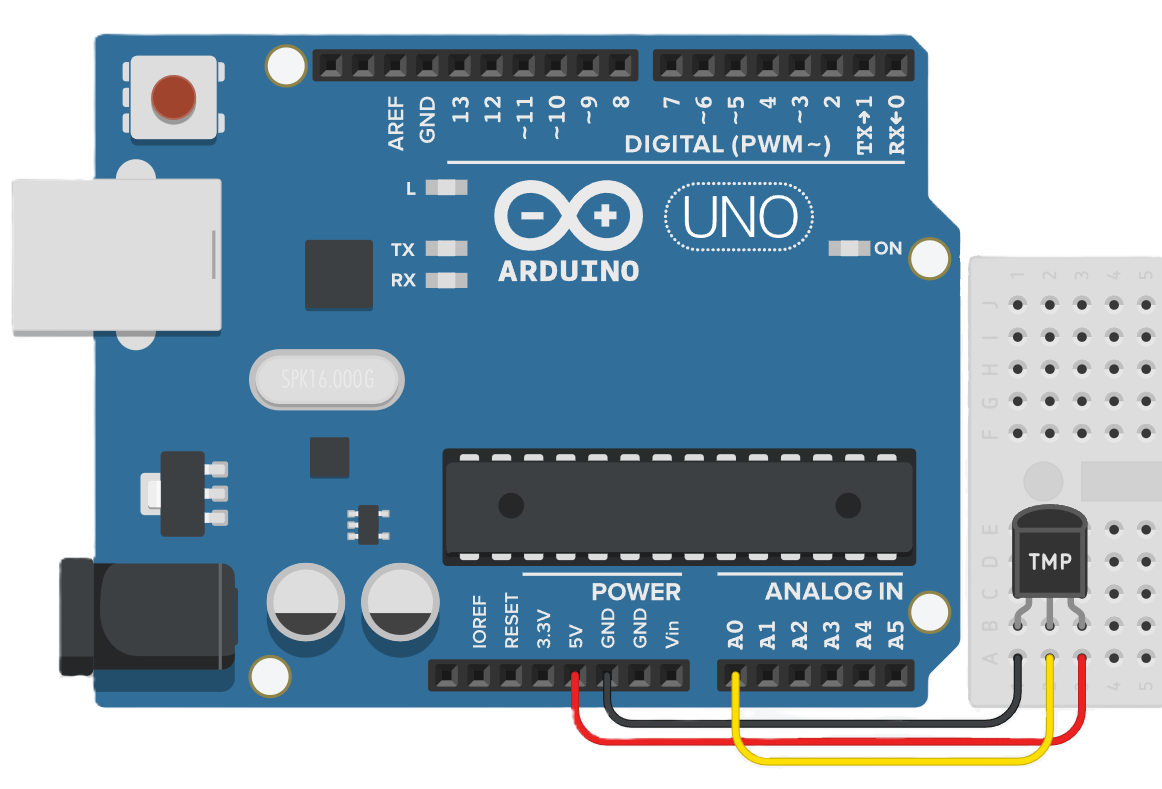
\includegraphics[width = \textwidth]{images/arduino/temp-pic.png}
                    \end{minipage}
                    \hfill
                    \begin{minipage}{0.49\textwidth}
                        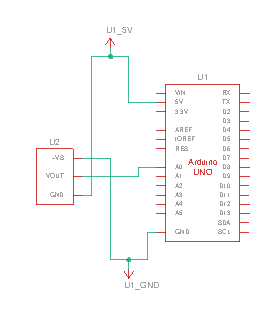
\includegraphics[width = \textwidth]{images/arduino/temp-scheme.pdf}
                    \end{minipage}
                    \caption{A sinistra una rappresentazione digitale del circuito realizzato per l'esperimento. A destra lo schema del circuito. Entrambe le illustrazioni sono state realizzate con Tinkercad\textsuperscript{\textregistered}.}
                    \label{fig:arduino-1}
            \end{figure}

            Per effettuare le misure ho usato il codice riportato di seguito. A intervalli di \SI{30}{\second} la lettura discreta di tensione data dal sensore\footnote{Come detto prima si tratta di un valore tra \num{0} e \num{1023}} e la converte in un numero decimale tra \SI{0}{\volt} e \SI{5}{V} attraverso la formula
            \begin{equation*}
                \frac{\text{\ttfamily (float)analogRead(SENSOR\_PIN)}}{\text{\ttfamily MAX\_READ}} * \text{\ttfamily MAX\_V}
                \mycomma
            \end{equation*}
            essendo $\text{\ttfamily MAX\_READ} = 1023$ e $\text{\ttfamily MAX\_V} = \SI{5}{\volt}$. Sapendo che a una tensione di \SI{0}{\volt} corrisponde una temperatura di \SI{0.5}{\celsius} e a \SI{4.5}{\volt} corrispondono \SI{100}{\celsius}, la conversione della lettura in gradi Celsius è data da
            \begin{equation}
                \bqty{\frac{\text{\ttfamily (float)analogRead(SENSOR\_PIN)}}{\text{\ttfamily MAX\_READ}} * \text{\ttfamily MAX\_V} - \text{\ttfamily A}} * \text{\ttfamily B}
                \mycomma
                \label{eq:ard:temp-conv}
            \end{equation}
            dove $\text{\ttfamily A} = \SI{0.5}{\volt}$ e $\text{\ttfamily B} = \SI{100}{\celsius\per\volt}$ sono i fattori di scala.

            La conversione dei valori discreti in temperatura è eseguita dal codice tra le righe \texttt{23} e \texttt{26} applicando la \eqref{eq:ard:temp-conv}. Vengono eseguite $\text{\ttfamily N} = 20$ misure consecuitive di cui è contestualmente calcolata la media che viene a sua volta stampata a schermo. Infine il codice attende il tempo mancante per raggiungere i \SI{30}{\second} dall'inizio del \txtloop.
            \lstinputlisting[language=C++]{code/arduino-temp.txt}

    \section{Dati}
        Attraverso il codice riportato al punto \S~\ref{ard:codice} ho misurato la temperatura della stanza ogni \SI{30}{s} per circa cinque ore e mezza; in \figref{fig:ard:raw-temp} sono riportati tutti i dati raccolti, avendo convertito il tempo in minuti.

        \begin{figure}
            \centering
            \begin{tikzpicture}
                \begin{axis}[
                    width       = \plotsize,
                    height      = 0.75\plotsize,
                    xlabel      = {Tempo (\unit{\min})},
                    ylabel      = {Temperatura (\unit{\celsius})},
                    xmin        = 0,  xmax = 330, xtick = {0,30,...,330},
                    ymin        = 16, ymax = 28,  ytick = {16,18,...,28},
                    tick align  = outside,
                    colorbar,
                    colormap/hot,
                    point meta  = y
                ]
                    \addplot+ [
                        scatter,
                        only marks,
                        mark        = *,
                        mark size   = 0.5pt,
                        scatter src = y,
                    ] table [
                        x index=0,
                        y index=1,
                        col sep=space
                        ] {code/python/temp_time_conv.dat};
                \end{axis}
            \end{tikzpicture}
            \caption{Andamento della temperatura nel tempo}
            \label{fig:ard:raw-temp}
        \end{figure}%
        \begin{figure}
            \centering
            \begin{tikzpicture}
                \begin{axis}[
                    width       = \plotsize,
                    height      = 0.75\plotsize,
                    xlabel      = {Tempo (\unit{\min})},
                    ylabel      = {Temperatura (\unit{\celsius})},
                    xmin        = 0,  xmax = 330, xtick = {0,30,...,330},
                    ymin        = 18, ymax = 26,  ytick = {18,...,26},
                    extra y ticks       = {24.5},
                    extra y tick labels = {\scriptsize{24.5}},
                    tick align  = outside,
                    legend pos  = south east
                ]
                    \addplot [
                        no marks,
                        draw    = black,
                    ] table [
                        x index = 0,
                        y index = 1,
                        col sep = space
                    ] {code/python/temp_avg.dat};
                    \addplot [
                        domain  = 0 : 330,
                        samples = 1000,
                        color   = red,
                        no marks
                    ] {24.5*(1 - exp(-((x+120)/95)))};
                    \draw[red, dashed] (0, 24.5) -- (330, 24.5);
                    \legend{Dati, Eq.~\eqref{eq:ard:temp-numerica}}
                \end{axis}
            \end{tikzpicture}
            \caption{Temperature mediate in intervalli di \SI{30}{\min}.}
            \label{fig:ard:avg-temp}
        \end{figure}

        \subsection{Prime considerazioni}
            Osservando il grafico si nota una evidente crescita di temperatura che, dopo una crescita regolare, oscilla fino a stabilizzarsi poco sopra i \SI{24}{\celsius}.
            
            I primi punti a temperatura più elevata possono essere dovuti a un precedente contatto con le mani e un riscaldamento del sensore che è poi tornato a temperatura ambiente. L'ampia oscillazione dei dati intorno ai \SI{130}{\min} deve essere dovuta a un movimento del sensore, che ho dovuto spostare di qualche centimetro. È quindi possibile che anche le successive oscillazioni siano dovute alla nuova posizione del sensore in un punto con un flusso d'aria più dinamico.

        \subsection{Breve analisi dei dati}
            Per per visualizzare il macro-andamento della temperatura tamponando il rumore, ho deciso di suddividere le misure in intervalli temporali di \SI{30}{\min} e riportare nel grafico in \figref{fig:ard:avg-temp} la temperatura media per ciascun intervallo.

            Anche in questo caso si notano l'andamento crescente della temperatura e il salto, ma le oscillazioni intorno alla temperatura finale di circa \SI{24}{\celsius} risultano smorzate. Si osserva inoltre che la temperatura si stabilizza intorno a questo valore \SI{150}{\min}---oppure  \SI{2}{\hour}\,\SI{30}{\min}---dopo l'accensione del riscaldamento.
            
            Svolgiamo adesso un fit dei dati di carattere prettamente qualitativo. Dal momento che il radiatore a regime avrà una temperatura $T^*$ fissata e, tenendo conto della dispersione del calore verso l'esterno, è ragionevole assumere che la temperatura della stanza $T\pqty{t}$ tenda asintoticamente a un valore finito $T_\text{f} \leq T^*$ per $t\to+\infty$. Una funzione crescente che ha un comportamento simile è
            \begin{equation}
                T\pqty{t} = T_\text{f}\bqty{1 - \exp\!\pqty{-\frac{t - t_0}{\tau}}}
                \mycomma
                \label{eq:ard:temp-analitica}
            \end{equation}
            per qualche valore di $T_\text{f}$, $t_0$ e $\tau$. Supponiamo arbitrariamente che la temperatura limite\footnote{I dati in \figref{fig:ard:raw-temp} oscillando superano i \SI{25}{\celsius} ma le ultime misure sono tutte comprese tra \SI{24}{\celsius} e \SI{24.5}{\celsius}, motivo per cui assumo quest'ultimo valore come temperatura limite.} sia $T_\text{f} = \SI{24.5}{\celsius}$; per quanto detto prima supponiamo inoltre che il tempo caratteristico\footnote{Dal momento che ``a occhio'' la temperatura di \SI{24.5}{\celsius} viene già raggiunta dopo \SI{150}{\min}, scegliamo il tempo caratteristico come il tempo necessario a raggiungere il \SI{63}{\%}, ovvero \textit{$\pqty{1/e}$-esimo} della temperatura finale.} sia $\tau = \SI{95}{min} \approx$ \SI{63}{\%} di \SI{150}{\min}. Imponendo che sia $T\pqty{0} = \SI{18.63}{\celsius}$ troviamo
            \begin{equation*}
                t_0
                = \tau \log\!\bqty{1-\frac{T\pqty{0}}{T_\text{f}}}
                \approx -\SI{135}{\min}
                \myperiod
            \end{equation*}

            Infine per centrare meglio la funzione rispetto agli intervalli di \SI{30}{\min} sommiamo a $t_0$ un valore di \SI{15}{\min}, pari a metà dell'intervallo di tempo. La funzione finale che si ottiene sostituendo questi valori nella \eqref{eq:ard:temp-analitica} e si trova rappresentata in \figref{fig:ard:avg-temp} è
            \begin{equation}
                T\pqty{t} =  24.5 \bqty{1 - \exp\!\pqty{-\frac{t + 120}{95}}}
                \myperiod
                \label{eq:ard:temp-numerica}
            \end{equation}

    \section{Conclusioni}
        I dati presi possono essere ulteriormente migliorati facendo maggiore attenzione a non toccare gli strumenti o uscendo dalla stanza e assicurandosi che la porta non venga mai aperta.

        Per avere informazioni più dettagliate sulla bontà del fit si potrebbe invece procedere applicando il metodo dei minimi quadrati per determinare i tre parametri $T_\text{f}$, $t_0$ e $\tau$. Per eseguire un fit con due parametri invece che tre, si può migliorare l'accuratezza su $T_\text{f}$ continuando a prendere dati il più a lungo possibile. Questo permetterebbe di fissare la temperatura limite con più sicurezza e di determinare $t_0$ e $\tau$ attraverso la linearizzazione della \eqref{eq:ard:temp-analitica} in
        \begin{equation*}
            \log\!\bqty{1-\frac{T\pqty{t}}{T_\text{f}}} = \frac{t_0}{\tau} - \frac{1}{\tau}t 
            \quad\iff\quad 
            y\pqty{t} = c_1\pqty{t_0,\tau} + c_2\pqty{t_0,\tau}t
            \myperiod
        \end{equation*}

        Si potrebbe inoltre provare a utilizzare funzioni diverse dalla \eqref{eq:ard:temp-analitica} nel fit per provare a modellare quantitativamente le oscillazioni che si verificano in prossimità della temperatura limite, possibilmente dovute a moti convettivi non del tutto smorzati dall'uso dei ventilatori indicati al punto \S~\ref{ss:ard:preparazione}.
        
        \chapter{Misura di resistenze con un multimetro digitale}\label{ch:mult}
    \lettrine[loversize=0.08, lines=2]{T}{ra le esperienze} svolte con il multimetro digitale riporto la misura delle resistenze di alcuni materiali, tra cui anelli metallici, il corpo umano e alcuni resistori.

    Ai resistori dedico una sezione più approfondita in quanto ho preso \num{50} misure su resistori distinti---ma teoricamente con resistenza uguale---per verificare la distribuzione delle misure di resistenza.

    \section{Il multimetro}
        Lo strumento utilizzato per l'interezza dell'esperienza è un multimetro digitale della serie \emph{DVM841} della \emph{Velleman\textsuperscript{\textregistered}} \cite{velleman-dvm841}. Il multimetro è in grado di misurare tensione e corrente continua e alternata, resistenza, frequenza e temperatura. Avendo una risoluzione di \num{2000} punti, il display del multimetro può visualizzare un massimo di \num{1999} unità.
    \section{Resistori}
        Il kit presenta $N = \num{50}$ resistori distinti---come quelli in \figref{fig:mul:resistore}---il cui codice colore restituisce un valore\footnote{Lo si può dedurre da qualunque legenda fedele allo standard IEC 60062.} teorico di $\SI{820}{\ohm} \pm \SI{5}{\%}$, ovvero \SI{820(40)}{\ohm}.
        \begin{figure}
            \centering
            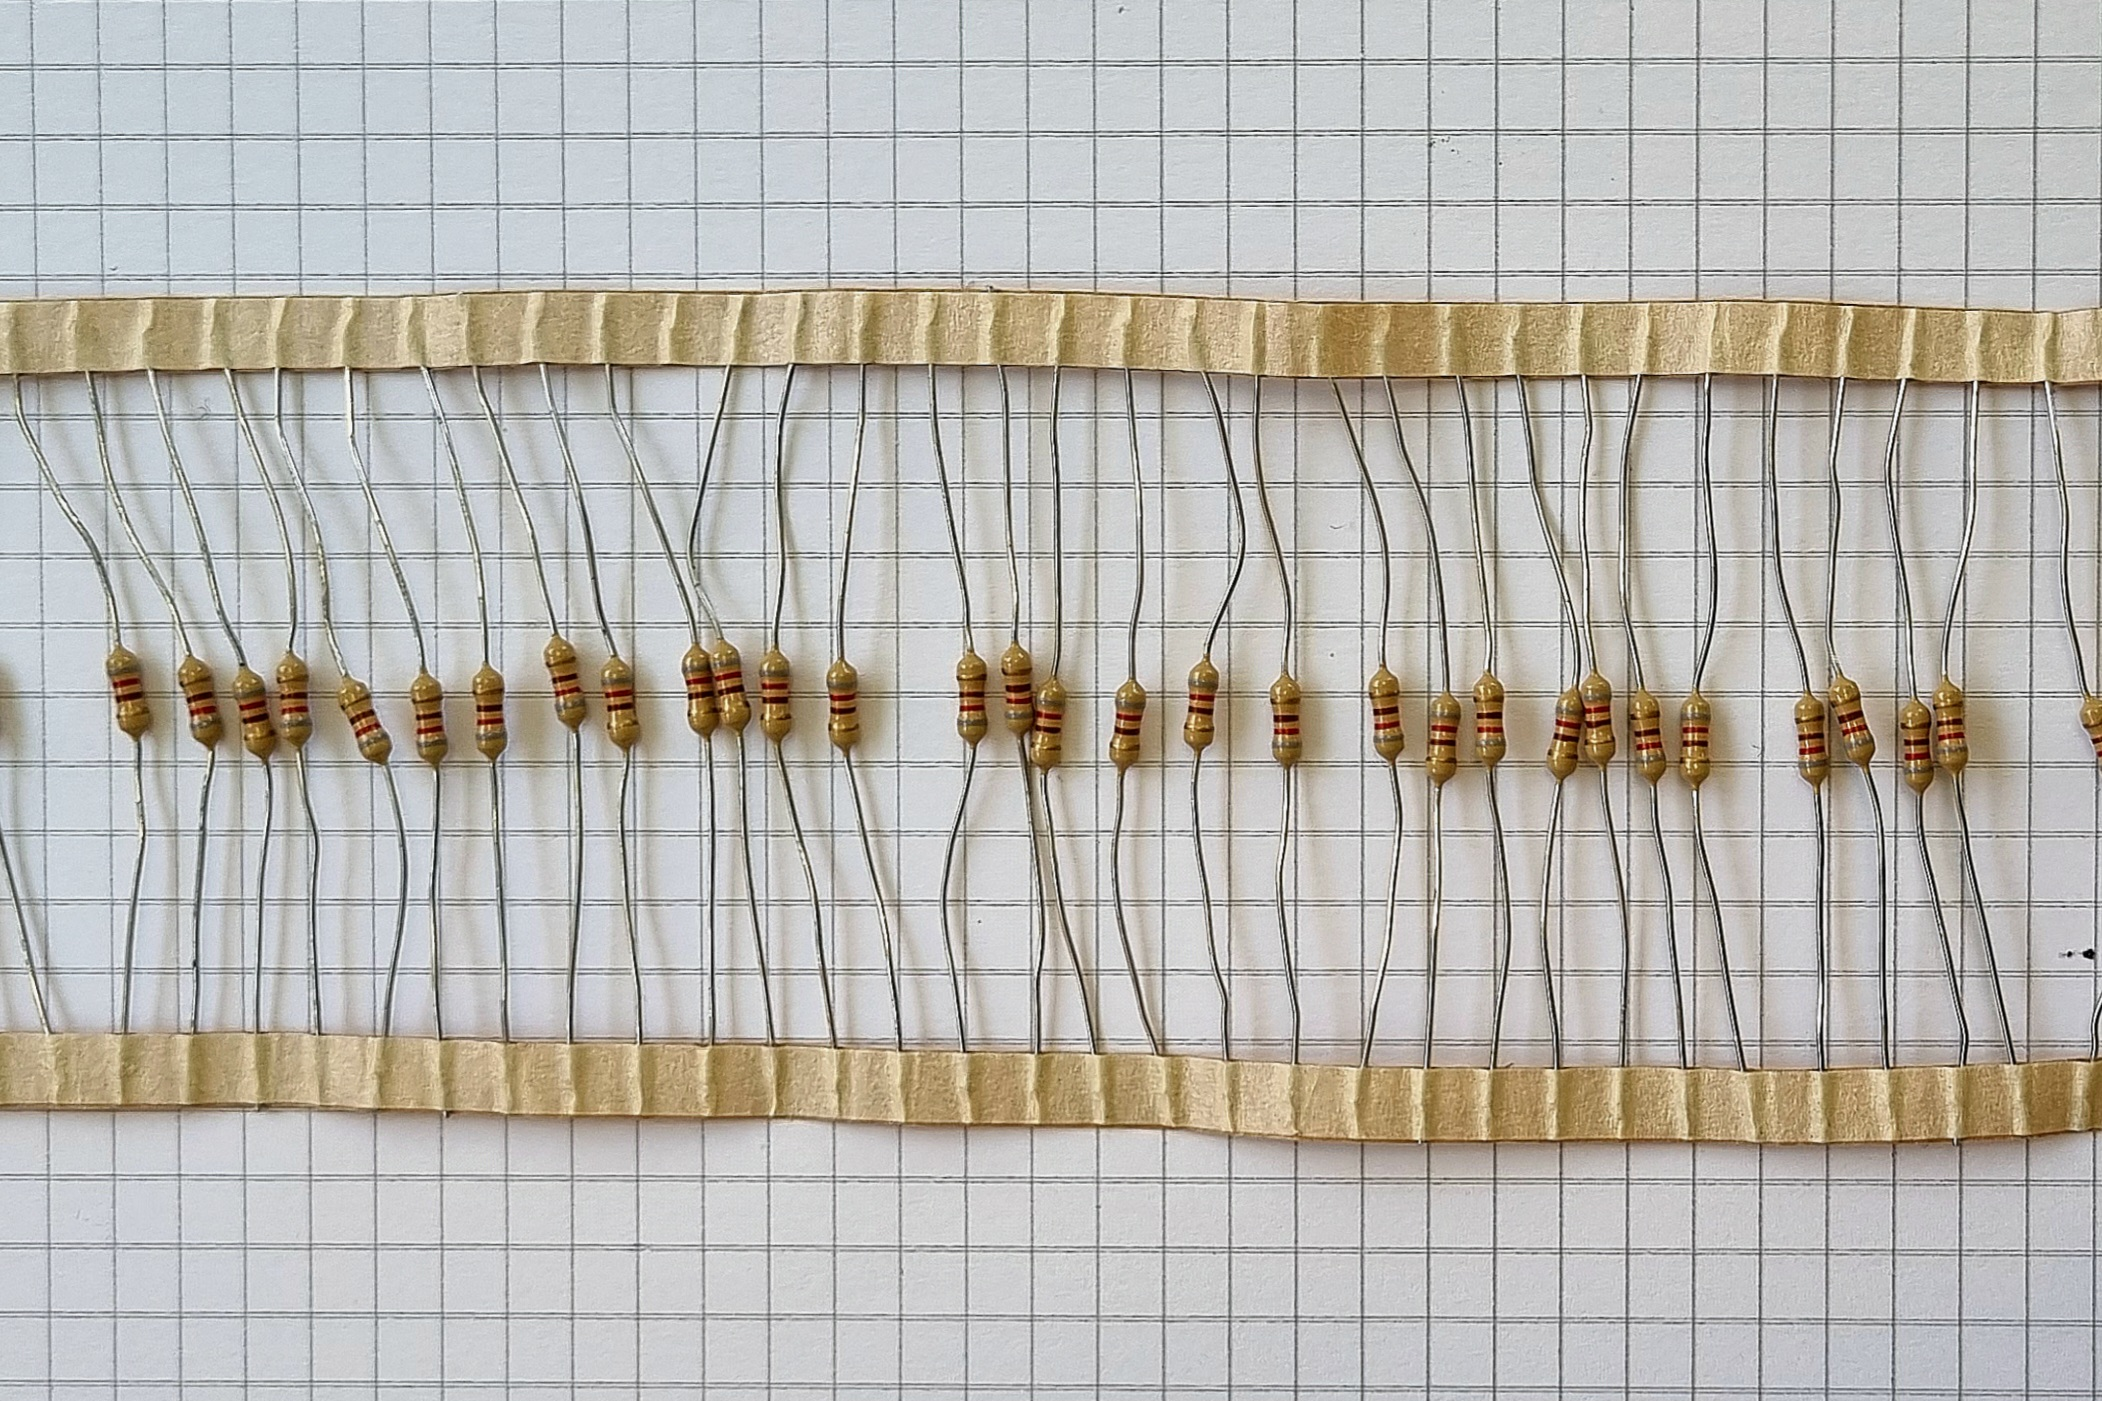
\includegraphics[width=0.4\textwidth]{images/multimetro/resistori.jpg}
            \hspace{0.05\textwidth}
            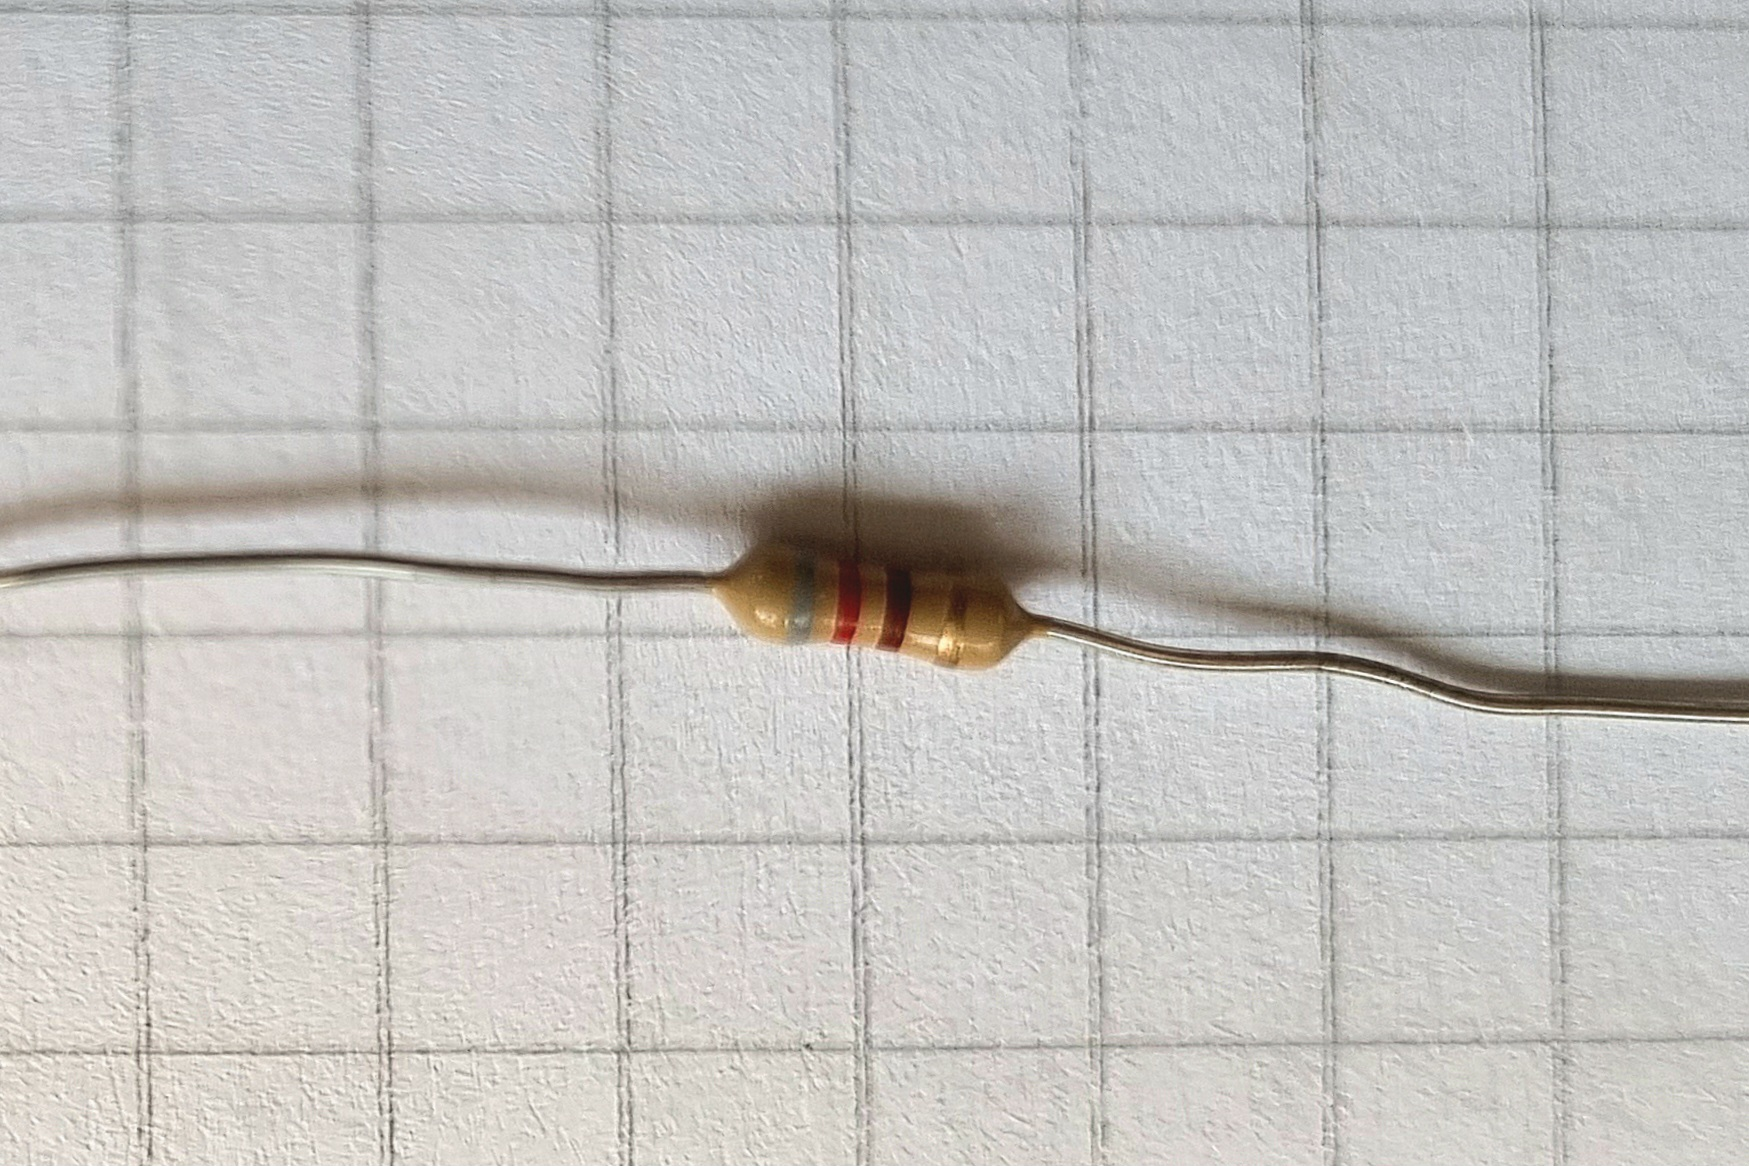
\includegraphics[width=0.4\textwidth]{images/multimetro/resistore.jpg}
            \caption{A sinistra alcuni dei \num{50} resistori da \SI{820}{\ohm}. A destra un dettaglio dove è visibile il codice colore.}
            \label{fig:mul:resistore}
        \end{figure}

        Ho effettuato le misure impostando il multimetro in modalità \emph{ohm}, alla portata di \SI{2}{\kilo\ohm}, poggiando i puntali sui terminali di ciascun resistore e aspettando di volta in volta che la lettura si stabilizzasse. I dati raccolti sono riportati in ordine crescente in \tabref{tab:mul:resistori}.
        \begin{table}
            \centering
            \begin{tabular}{cccccccccc}
    \hline
    \multicolumn{10}{c}{Resistenze (\unit{\ohm})}\\\hline\hline
    797 & 806 & 806 & 807 & 807 & 807 & 807 & 807 & 807 & 807 \\
    807 & 808 & 808 & 808 & 808 & 808 & 808 & 808 & 808 & 808 \\
    808 & 808 & 808 & 809 & 809 & 809 & 809 & 809 & 809 & 809 \\
    809 & 809 & 809 & 809 & 809 & 809 & 810 & 810 & 810 & 810 \\
    810 & 810 & 810 & 811 & 811 & 812 & 812 & 812 & 812 & 813 \\ \hline
\end{tabular}
            \caption{Misure di resistenza effettuate su \num{50} resistori distinti.}
            \label{tab:mul:resistori}
        \end{table}

        \subsection{Considerazioni preliminari}
            Notiamo subito che la resistenza media è $R_\text{m} = \SI{808.6}{\ohm}$ con una deviazione standard di $\sigma = \SI{2.3}{\ohm}$, l'errore sul valor medio è quindi $\sigma_R = \sigma / \sqrt{N-1} = \SI{0.33}{\ohm}$, che è confrontabile con la sensibilità dello strumento di \SI{1}{\ohm}.
            
            Questi valori rientrano completamete nell'intervallo fornito dal costruttore; tuttavia, il fatto che tutte le misure siano inferiori a \SI{820}{\ohm} suggerisce la presenza di un errore sistematico.\footnote{Se si trattasse di errori casuali dovuti a imprecisioni di fabbricazione, mi aspetterei letture sia al di sopra che al di sotto del valore di riferimento; è poco probabile che tutte le resistenze devino dal valore teorico allo stesso modo a meno che non si sia verificato un evento che ha alterato tutte le resistenze---un lotto prodotto con lo stesso materiale meno resistente, seppur entro il margine del \SI{5}{\%}, o deterioramento nel tempo.}

            Il dato di resistenza minima di \SI{797}{\ohm} può essere scartato secondo il cirerio di Chauvenet. Esso dista più di $4\sigma$ dal valor medio (ca. $\num{4.17}\sigma$) e il numero di dati atteso\footnote{Per il calcolo di questa probabilità ho fatto riferimento a [INSERIRE TAYLOR!!!]} su un campione di $N = 50$ elementi a una distanza maggiore o uguale a $4\sigma$ è pari a $\num{0.003} \ll 1/2$. Scartando questo dato la nuova media e la nuova deviazione standard sono:

        \subsection{Test del $\chi^2$}
            Supponiamo che le misure seguano la distribuzione normale centrata in $R_\text{m}$ e di ampiezza $\sigma$:
            \begin{equation*}
                N\pqty{x; R_\text{m}, \sigma}
                = \frac{1}{\sqrt{2\pi\sigma^2}} \exp[ -\frac{1}{2}\pqty{\frac{x - R_\text{m}}{\sigma}}^2]
                \myperiod
            \end{equation*}
            
            Costruiamo quindi un istogramma dei dati. Visto l'intervallo contenuto in cui le misure variano, ho scelto di raccogliere i dati in bin di ampiezza \SI{1}{\ohm}, uno per ciascun valore misurato; ciascun bin si estende da mezza unità \emph{prima} del valore di interesse a mezza unità \emph{dopo}. In \tabref{tab:mul:bin-istogramma} sono riportati i bin e le frequenze osservate $O_k$.
            \begin{table}
                \centering
                \begin{tabular}{ccccc|rc}\hline
    \multicolumn{5}{c}{Intervalli}                  & $O_k$    & $E_k$       \\
    \hline\hline
                  &     & $R$ & $<$ & $\num{806.5}$ & \num{2}  & \num{4.133} \\
    $\num{806.5}$ & $<$ & $R$ & $<$ & $\num{807.5}$ & \num{8}  & \num{5.735} \\
    $\num{807.5}$ & $<$ & $R$ & $<$ & $\num{808.5}$ & \num{12} & \num{6.925} \\
    $\num{808.5}$ & $<$ & $R$ & $<$ & $\num{809.5}$ & \num{13} & \num{7.278} \\
    $\num{809.5}$ & $<$ & $R$ & $<$ & $\num{810.5}$ & \num{6}  & \num{6.655} \\
    $\num{810.5}$ & $<$ & $R$ & $<$ & $\num{811.5}$ & \num{2}  & \num{5.297} \\
    $\num{811.5}$ & $<$ & $R$ & $<$ & $\num{812.5}$ & \num{4}  & \num{3.668} \\
    $\num{812.5}$ & $<$ & $R$ &     &               & \num{1}  & \num{2.211} \\
    \hline
\end{tabular}
                \caption{Suddivisione dei dati per il test del $\chi^2$. Ometto le unità di misura per chiarezza espositiva e semplicità dei calcoli.}
                \label{tab:mul:bin-istogramma}
            \end{table}

            Da qui eseguo il test nell'usuale modo: converto gli esetremi dell'intervallo in variabili normali standardizzate sottraendo la media e dividendo per la deviazione standard, attraverso un foglio di calcolo trovo il valore dell'integrale della gaussiana per ciascun intervallo, moltiplico tale valore per la dimensione del campione $N = 49$ per trovare i valori attesi $E_k$.
        \chapter{Accettanza geometrica di un Rivelatore}\label{ch:acc}
    \lettrine[loversize=0.08, lines=2]{L}{'ultima esperienza} consiste nel calcolare l'accettanza geometrica di un rivelatore, definita come il rapporto tra il numero di particelle incidenti e il numero di particelle emesse, sfruttando la generazione di numeri casuali e il metodo Montecarlo.

    \section{Il sistema fisico proposto}
        L'obiettivo che mi sono posto è stato quello di calcolare l'accettanza geometrica di un rivelatore a forma di dischetto con raggio variabile, posto in una posizione arbitraria nel semispazio positivo delle $z$. In modo analogo, la sorgente di radiazioni è costituita da un secondo dischetto, anch'esso con raggio variabile, centrato nell'origine.

        Le ipotesi che ho fatto sono le seguenti:
        \begin{enumerate}
            \item Ciascun punto della sorgente emette in maniera isotropa, ovvero in tutte le direzioni con la stessa probabilità;
            \item La probabilità di emissione da parte di un punto della sorgente è uniforme, ovvero tutti i punti hanno la stessa probabilità di emettere una particella;
            \item Il rivelatore e la sorgente sono sempre paralleli tra loro e al piano $Oxy$, e il rivelatore è sempre posto sopra la sorgente.
        \end{enumerate}

        Per ragioni di simmetria, la posizione del rivelatore sopra la sorgente non causa alcuna perdita di generalità. Se il rivelatore avesse altezza $z=0$, visto lo spessore nullo sia della sorgente che del rivelatore, nessuna particella verrebbe rivelata. La sorgente inoltre emette in modo simmetrico rispetto al piano $Oxy$, quindi il caso $z<0$ è equivalente al caso $z>0$.

        \subsection{Sorgente puntiforme}\label{ss:acc:sorgente-puntiforme}
            Dal momento che la sorgente può emettere da un solo punto alla volta, cominciamo col risolvere il problema nel caso di una sorgente puntiforme nell'origine e un rivelatore che può essere spostato rispettando le ipotesi di cui sopra. 
            
            Affinché la distribuzione delle particelle sia uniforme, generare delle coordinate cartesiane casuali non è sufficiente. La scelta che ho fatto è quella di generare delle \emph{direzioni} casuali in coordinate sferiche $\pqty{\varrho,\vartheta,\varphi}$, risparmiando la spesa computazionale di generare la distanza $\varrho$ dall'origine. Per le proprietà delle coordinate sferiche possiamo generare uniformemente $\cos\!\vartheta\in\left]-1;1\right[$, per poi ricavare $\vartheta$ prendendone l'arcocoseno, mentre possiamo generare uniformemente $\varphi\in\left[0;2\pi\right[$.

            Fissata una direzione $\pqty{\vartheta,\varphi}$, la particella emessa dalla sorgente si muoverà lungo la retta che passa per l'origine avente tale direzione. Ci chiediamo quindi se questa retta intersecherà il rivelatore, e, in caso affermativo, in quale punto.\footnote{Sapere il punto non è necessario per il calcolo dell'accettanza geometrica, ma è utile allo scopo di generare un'immagine del sistema.}

            Da semplici considerazioni geometriche, se indichiamo con $P\equiv\pqty{x,y,z}$ il generico punto dello spazio, con $C\equiv\pqty{x_c,y_c,z_c}$ il centro del rivelatore e con $R$ il suo raggio, il punto appartiene al dischetto se si verificano contemporaneamente le seguenti condizioni:
            \begin{align}
                \pqty{P - C}^2 &\leq R^2 \mycomma
                \label{eq:acc:cond-1}
                \\
                z &= z_c \myperiod
                \label{eq:acc:cond-2}
            \end{align}
            La prima condizione corrisponde a $\pqty{x - x_c}^2 + \pqty{y - y_c}^2 + \pqty{z - z_c}^2 \leq R^2$, che messa a sistema con la seconda dà $\pqty{x - x_c}^2 + \pqty{y - y_c}^2 \leq R^2$. Passiamo quindi in coordinate polari per trovare le condizioni che devono rispettare i valori di $\vartheta$ e $\varphi$:
            \begin{equation*}
                \begin{cases}
                    x = \varrho\sin\!\vartheta\cos\!\varphi \\
                    y = \varrho\sin\!\vartheta\sin\!\varphi \\
                    z = \varrho\cos\!\vartheta
                \end{cases}
                \myperiod
            \end{equation*}
            Sostituendo queste relazioni nella condizione di appartenenza al cerchio troviamo:
            \begin{equation*}
                \pqty{\varrho\sin\!\vartheta\cos\!\varphi - x_c}^2 + \pqty{\varrho\sin\!\vartheta\sin\!\varphi - y_c}^2 \leq R^2
                \mycomma
            \end{equation*}
            che con qualche passaggio si riduce a
            \begin{equation*}
               \varrho^2 \sin\!^2\vartheta + x_c^2 + y_c^2 - 2 \varrho\sin\!\vartheta\pqty{x_c\cos\!\varphi + y_c\sin\!\varphi} \leq R^2
               \mycomma
            \end{equation*}
            che a sua volta, a patto di porre $x_c = d\cos\!\varphi_c$, $y_c = d\sin\!\varphi_c$ e di conseguenza $x_c^2 + y_c^2 = d^2$, non è altro che il teorema del coseno applicato al triangolo formato dalle proiezioni sul piano $Oxy$ dei punti $O$, $P$ e $C$, che ha un angolo in $O$ proprio pari a $\varphi - \varphi_c$:
            \begin{equation}
                \varrho^2 \sin\!^2\vartheta + d^2 - 2 \varrho\sin\!\vartheta d \cos\!\pqty{\varphi - \varphi_c} \leq R^2
                \myperiod
                \label{eq:acc:cond-rho}
            \end{equation}
            Se assumiamo $\cos\!\vartheta \neq 0$---che è vero se $P \notin Oxy$, e ciò non è restrittivo in quanto il piano è un sottoinsieme a misura nulla dello spazio $\R^3$---possiamo invertire la \eqref{eq:acc:cond-2} scritta in coordinate polari per esplicitare $\varrho$:
            \begin{equation}
                \varrho = \frac{z_c}{\cos\!\vartheta}
                \myperiod
                \label{eq:acc:rho-expl}
            \end{equation}
            Sostituendo quest'ultima relazione \eqref{eq:acc:rho-expl} nella \eqref{eq:acc:cond-rho} si ottiene
            \begin{equation}
                z_c \tan\!\vartheta + d^2 - 2 z_c \tan\!\vartheta d \cos\!\pqty{\varphi - \varphi_c} \leq R^2
                \myperiod
                \label{eq:acc:diseq}
            \end{equation}

            I valori $z_c$, $d$ e $\varphi_c$ sono costanti, per cui una volta generati $\vartheta$ e $\varphi$ è sufficiente verificare la disequazione per sapere se il raggio interseca o no il rivelatore.
            
            Resta quindi da trovare esplicitamente la posizione dei punti $P^*\equiv\pqty{x^*, y^*, z^*}$ che soddisfano le condizioni di appartenenza al cerchio. La quantità $z_c \tan\!\vartheta$ è la proiezione del segmento $\overline{OP^*}$ sul piano $Oxy$: il suo prodotto per $\cos\!\varphi$ e $\sin\!\varphi$ ci dà rispettivamente le coordinate $x^*$ e $y^*$. L'altezza $z^*$ è naturalmente la stessa del rivelatore $z_c$. Possiamo dunque scrivere
            \begin{equation*}                
                P^*\equiv z_c \pqty{\tan\!\vartheta \cos\!\varphi, \tan\!\vartheta \sin\!\varphi, 1}
                \myperiod
            \end{equation*}
            
            È importante notare che il problema non distingue tra ``sopra'' e ``sotto'', per cui un raggio rivolto verso il simmetrico di $P^*$ rispetto all'origine sarà ugualmente soluzione della disequazione. Ho comunque deciso di conservare tali punti in modo da raddoppiare la risoluzione del metodo; per compensare l'effetto basterà dividere per $2$ il conteggio finale dei punti che intersecano il rivelatore nel calolo dell'accettanza geometrica.

        \subsection{Sorgente estesa}
            Per estendere quanto sviluppato al punto precedente alla sorgente estesa, è sufficiente fare una semplice traslazione: generato un punto $S\equiv\pqty{x_s, y_s, 0}$ arbitrario nella sorgente circolare, è possibile calcolare la posizione relativa del centro $C'$, nel sistema di riferimento che ha il cento in $S$, che avrà quindi coordinate $C'\equiv\pqty{x_c - x_s, y_c - y_s, z_c}$. Fatto ciò possiamo generare una direzione casuale e, con gli stessi passaggi del punto precedente, trovare gli eventuali punti di intersezione nel sistema di riferimento del punto sorgente. Trovati tali punti, sarà immediato riportarli nel sistema di riferimento del centro della sorgente con la traslazione inversa. Si trova in particolare
            \begin{equation*}
                \begin{cases}
                    x^* = x_s + z_c\tan\!\vartheta\cos\!\varphi \\
                    y^* = x_s + z_c\tan\!\vartheta\sin\!\varphi \\
                    z^* = z_c
                \end{cases}
                \mycomma
            \end{equation*}
            dove $\vartheta$ e $\varphi$ sono ancora le direzioni generate casualmente nel sistema del punto sorgente; $z_c$ resta invariato dal momento che il punto $S$ giace ancora in $Oxy$.
    
    \section{Codice e generazione dei punti}
        Come per la simulazione dell'assorbimento di particelle cariche esposto al Capitolo \Sref{ch:bet}, anche per questo progetto l'interezza del codice è reperibile sul mio profilo GitHub.\footnote{Repository: \url{https://github.com/ImAure/geometric-acceptance}}

        Il programma può essere lanciato scegliendo fin da subito il numero di punti da generare, le dimensioni della sorgente e del rivelatore e la posizione di quest'ultimo. Dopo aver verificato la validità dell'input e caricati i dati in memoria, il programma genera un punto casuale come sorgente in coordinate polari piane e una direzione casuale per la radiazione in coordinale polari sferiche.
        \lstinputlisting[style = CStyle]{code/accettanza/random.txt}
        Affinché la distribuzione sia uniforme, nel caso bidimensionale viene generato uniformemente $\varrho^2 \in \bqty{0;1}$, ne viene presa la radice quadrata e il risultato è moltiplicato per il raggio massimo. Nel caso tridimensionale la funzione fa la stessa cosa con $\varrho^3$ e la radice terza, mentre come detto prima viene generato\footnote{Per essere precisi, il coseno è generato tra \num{1} e \num{-1} piuttosto che tra \num{-1} e \num{1}. Questo perché per $\vartheta = 0$ si ha $\cos\!\vartheta = \num{1}$ e per $\vartheta = \pi$ si ha $\cos\!\vartheta = \num{-1}$} $\cos\!\vartheta \in \left]-1;1\right[$ e ne viene preso l'arcocoseno per ricavare $\vartheta$.

        Entrambe le funzioni ammettono come input anche un raggio massimo negativo: in quel caso il raggio verrà posto uguale a $1$ e verrà generata casualmente solo la direzione. Questo comportamento è sfruttato nella generazione casuale della radiazione, in cui la chiamata a funzione avviene come \verb|rand_polar3D(&ray, -1)|.
        
        La funzione \verb|intercept()| verifica l'intersezione del raggio nel caso di una sorgente puntiforme posta nell'origine. Per utilizzarla correttamente viene calcolata la posizione relativa del rivelatore $\pqty{x_c', y_c', z_c}$ e questa viene data in input alla funzione insieme alla direzione da verificare.
        \lstinputlisting[style = CStyle]{code/accettanza/intercept.txt}
        La funzione valuta quindi la disequazione \eqref{eq:acc:diseq} e in caso di successo aggiorna il conteggio e stampa su file le coordinate del punto di partenza e del punto di arrivo, dopo averle riportate di nuovo nel riferimento del centro della sorgente.

        Sullo stesso file, la funzione \verb|intercept()| si occupa anche di stampare la posizione dei punti di intersezione del rivelatore convertendoli in coordinate polari nel sistema di riferimento centrato nel rivelatore stesso. Questi ultimi dati possono essere usati per costruire un istogramma e apprezzare la non uniformità della distribuzione della radiazione sul sensore.

        L'accettanza geometrica del rivelatore è infine calcolata dividendo il numero di raggi che intersecano il rivelatore per il numero totale di raggi generati. Come giustificato alla fine del punto \Sref{ss:acc:sorgente-puntiforme}, questo numero è a sua volta diviso per \num{2} per tenere conto solo dei raggi che viaggiano nel semispazio $z > 0$; analogamente il numero \verb|hits|, prima di essere stampato a schermo, è diviso per \num{2} e arrotondato. Il programma quindi stampa a schermo anche l'accettanza geometrica del rivelatore e l'equivalente angolo solido che esso sottende.

    \section{Esempi e immagini}
        Riporto qui degli esempi di esecuzione della simulazione. Il nome dell'eseguibile è \verb|sim|, mentre gli argomenti che compaiono sono, in ordine: il numero di punti da generare $N$, il raggio della sorgente, le coordinate $\pqty{x,y,z}$ del centro del rivelatore, il suo raggio $R$ e la stringa da usare per i nomi dei file in cui salvare tutti i punti generati e i punti da graficare. I nomi dei file saranno rispettivamente \verb|<string>.1.txt| e \verb|<string>.2.txt|.

        Le immagini sono generate tramite uno script python che estrae i numeri dal secondo file. La prima parte del programma rappresenta i punti di partenza dei raggi in rosso e i punti di arrivo in verde, collegandoli con una riga grigia; la seconda parte del programma crea un istogramma in tre dimensioni i cui bin sono settori di corone circolari.
        
        Volendo un numero di bin che sia circa uguale a $\sqrt{N}$, gli intervalli $\bqty{0;R}$ e $\bqty{0;2\pi}$ andrebbero divisi ciascuno in $\lfloor\sqrt[4]{N}\rfloor$ sottointervalli, in questo modo il numero di bin sarebbe proprio $\lfloor\sqrt[4]{N}\rfloor\lfloor\sqrt[4]{N}\rfloor \simeq \sqrt{N}$. Dal momento che però in questo modo venivano generate barre troppo sottili e con altezze molto variabili, ho scelto di usare $\sqrt[5]{N}$ al posto di $\sqrt[4]{N}$. I bin sono inoltre generati in modo da avere area costante: viene diviso l'intervallo $\bqty{0;1}$ uniformemente in $\lfloor\sqrt[5]{N}\rfloor$ intervalli, viene presa la radice quadrata dei valori degli estremi e infine viene tutto moltiplicato per $R$. L'altezza delle barre invece è pari alla densità di frequenza ottenuta dividendo la frequenza relativa associata al bin per l'area del bin stesso.

        \begin{figure}[ht]
            \textbf{Sorgente piccola e rivelatore allineato}
            \lstinputlisting[style = mybash]{code/accettanza/bash1.txt}
            \centering
            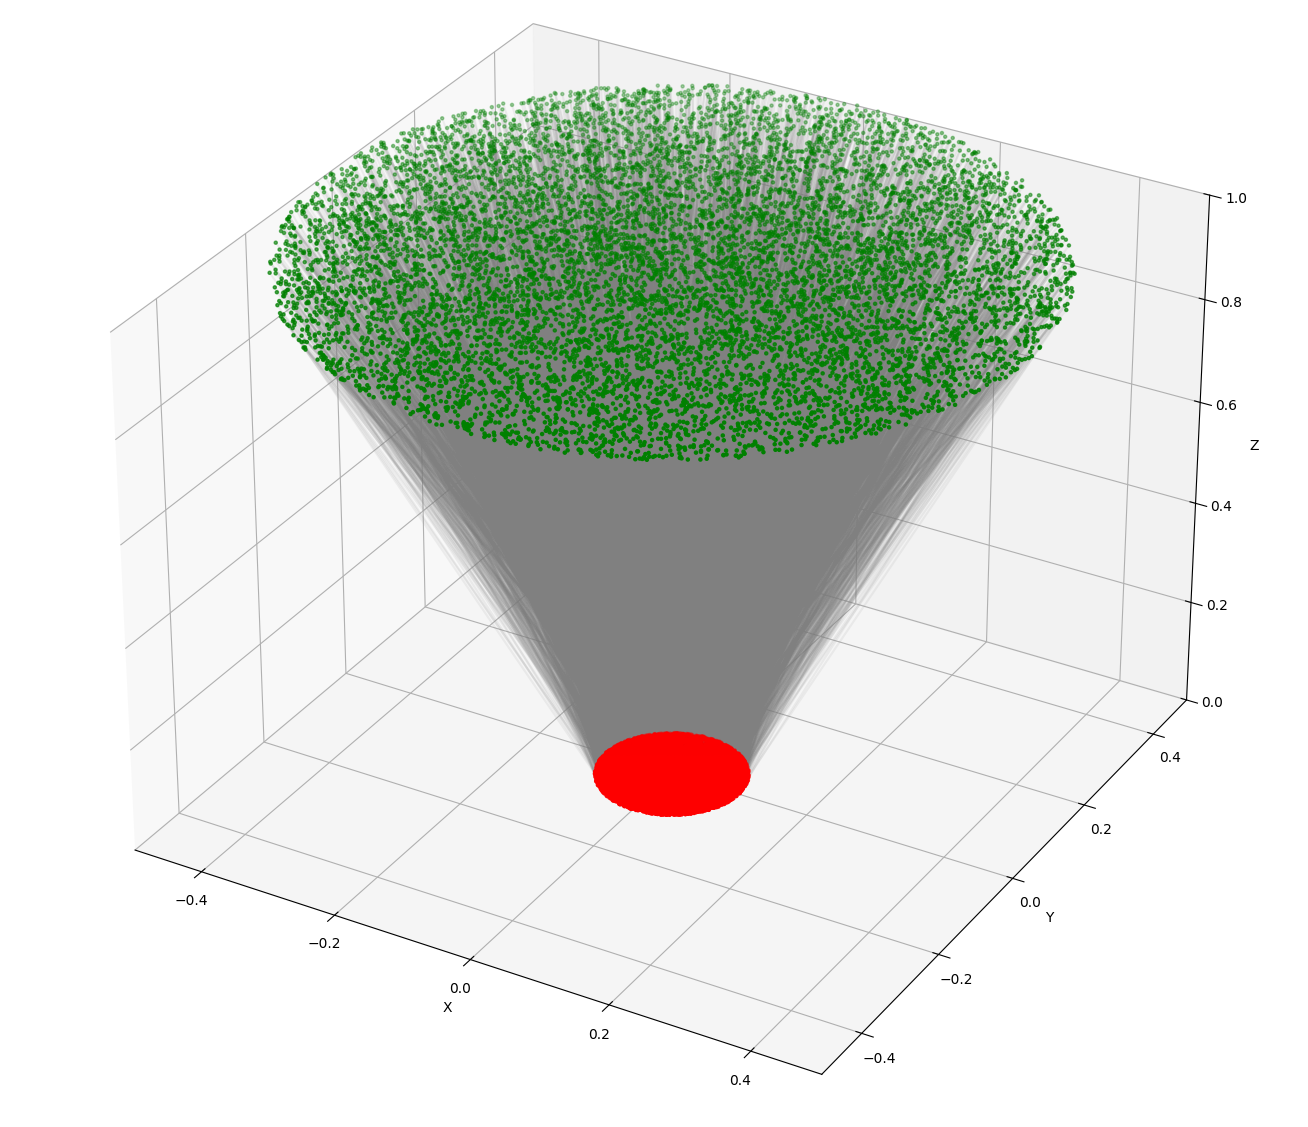
\includegraphics[width=0.49\textwidth]{images/accettanza/example1.1.png}
            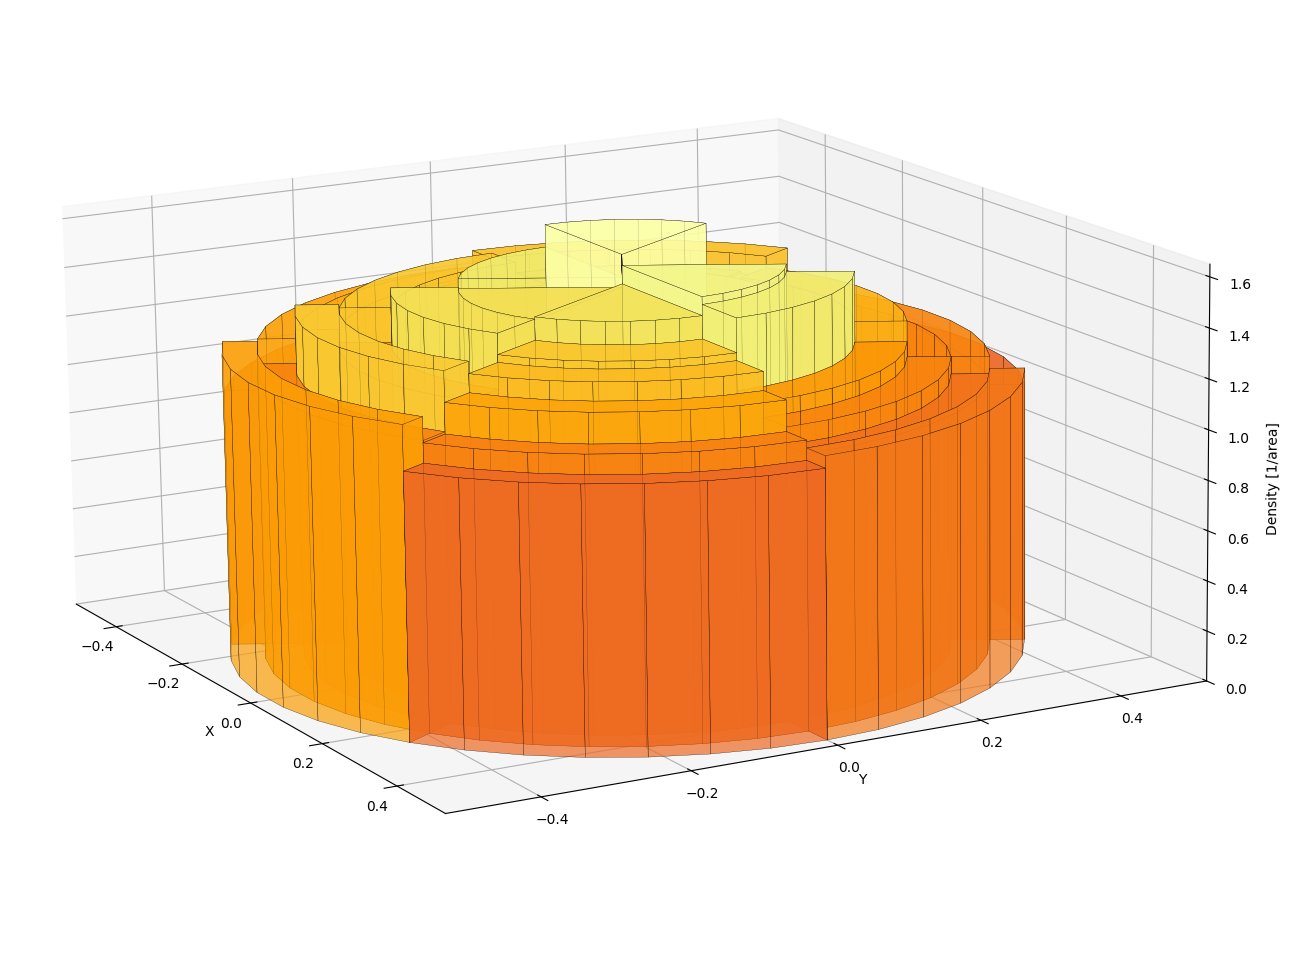
\includegraphics[width=0.49\textwidth]{images/accettanza/example1.2.png}
            \caption{Notiamo dall'istogramma che la distribuzione è maggiormente concentrata al centro.}
        \end{figure}

        \begin{figure}[ht]
            \textbf{Sorgente puntiforme e rivelatore traslato}
            \lstinputlisting[style = mybash]{code/accettanza/bash2.txt}
            \centering
            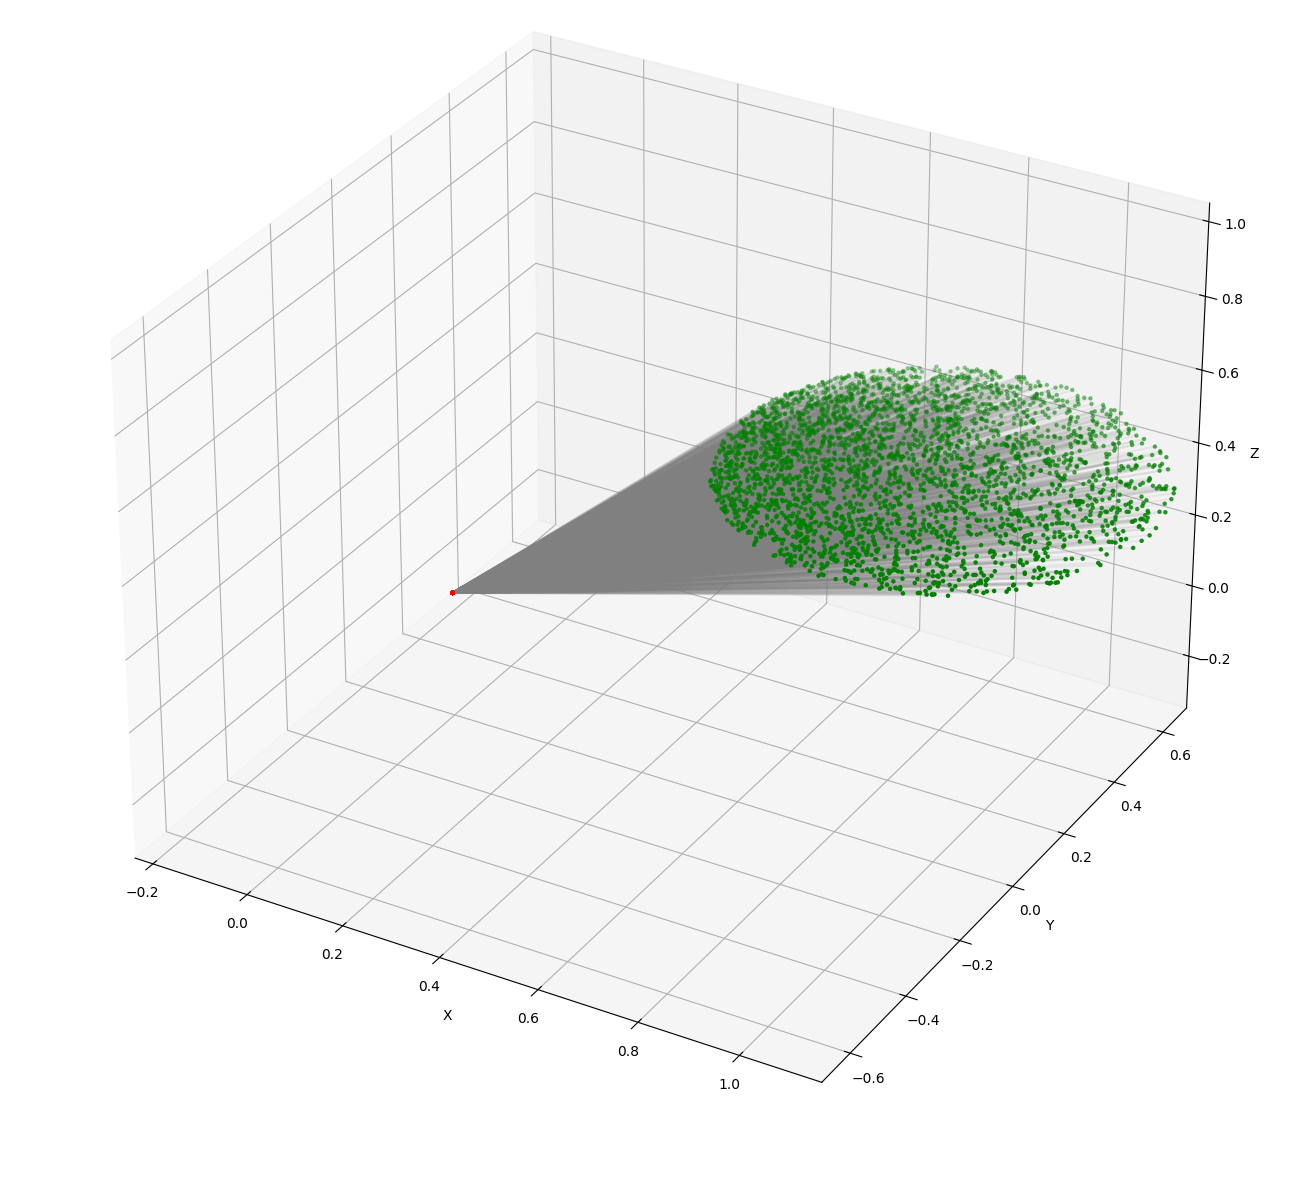
\includegraphics[width=0.49\textwidth]{images/accettanza/example2.1.png}
            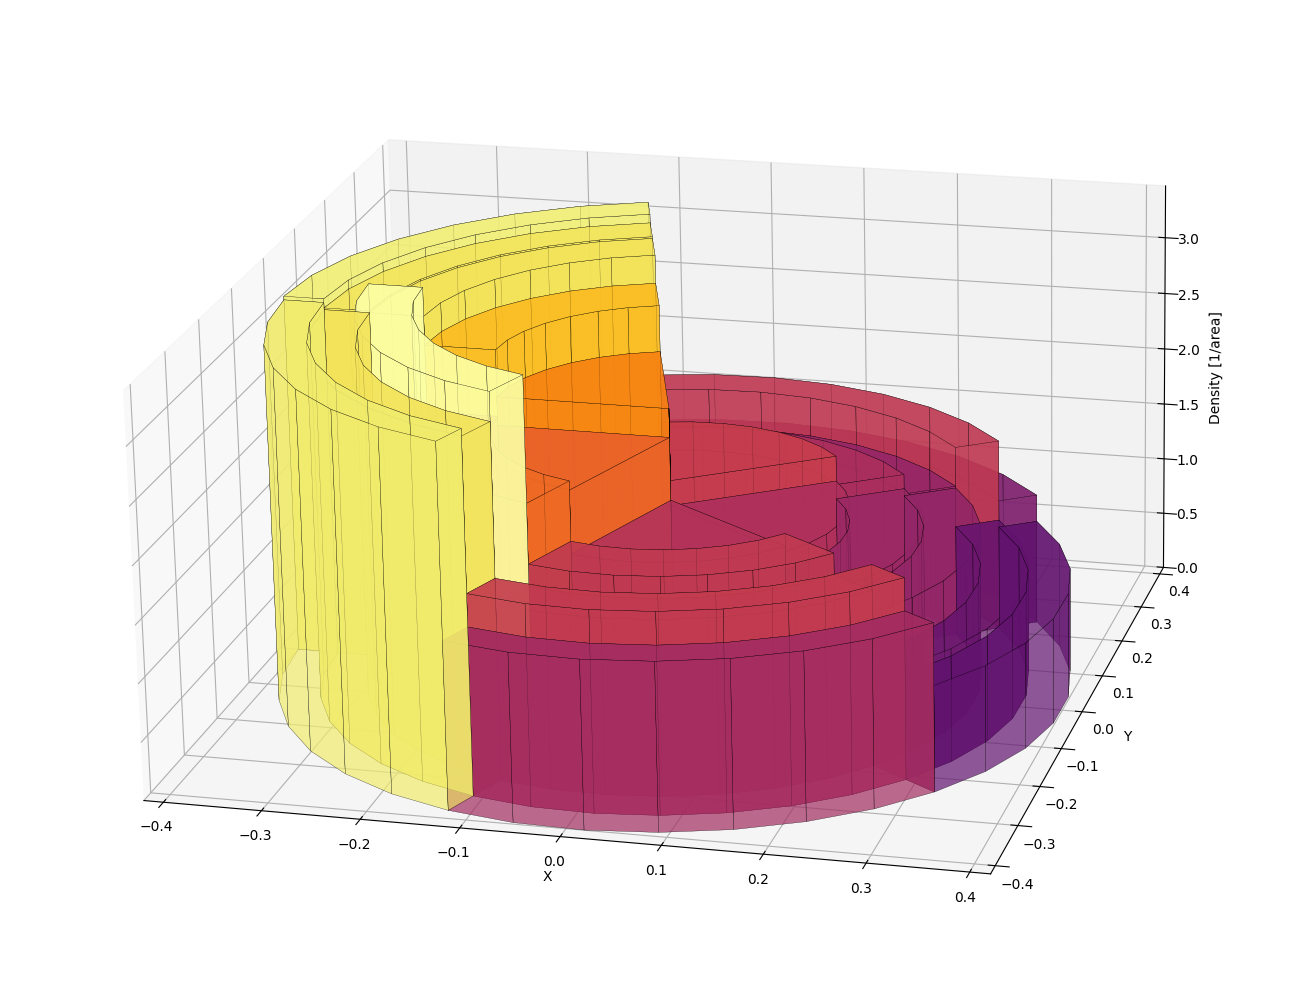
\includegraphics[width=0.49\textwidth]{images/accettanza/example2.2.png}
            \caption{In questo caso osserviamo come la radiazione sia particolarmente concentrata sul lato del rivelatore più vicino alla sorgente.}
        \end{figure}
        
        \begin{figure}[ht]
            \textbf{Sorgente e rivelatore confrontabili}
            \lstinputlisting[style = mybash]{code/accettanza/bash3.txt}
            \centering
            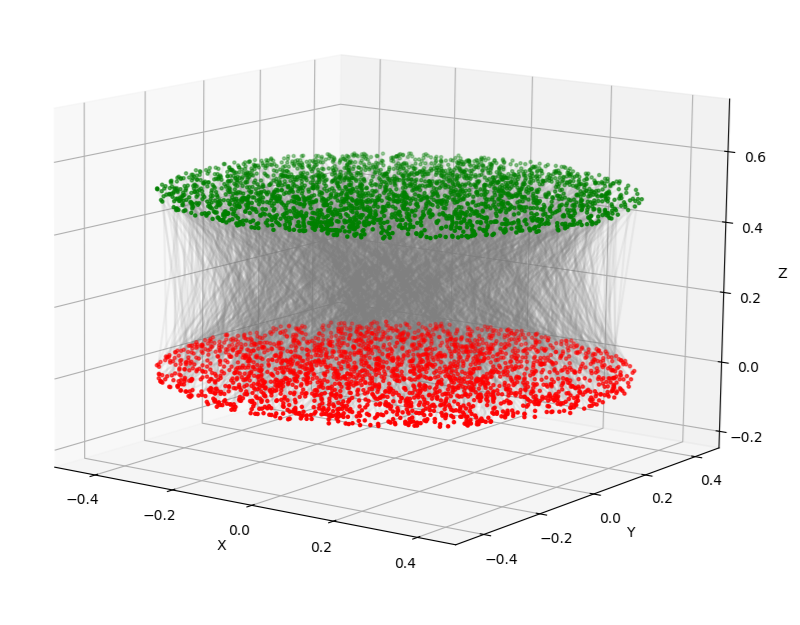
\includegraphics[width=0.49\textwidth]{images/accettanza/example3.1.png}
            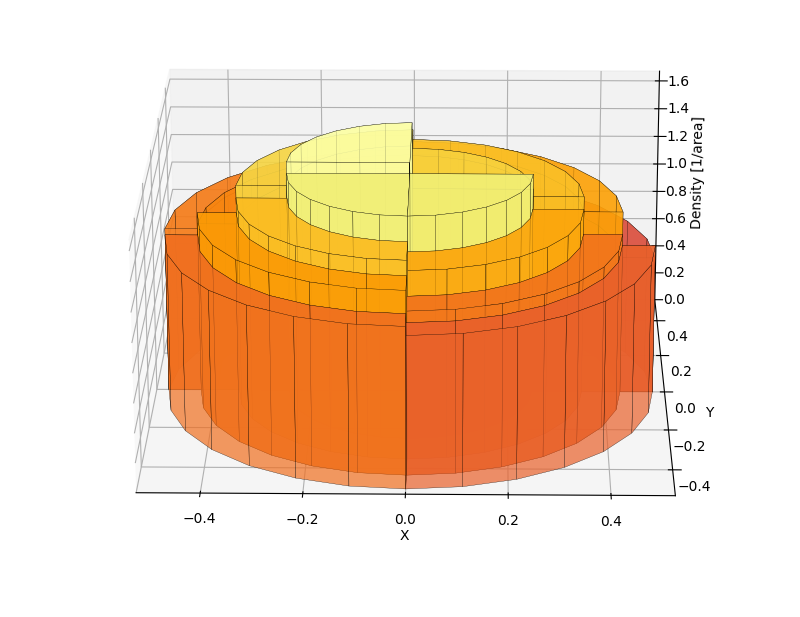
\includegraphics[width=0.49\textwidth]{images/accettanza/example3.2.png}
            \caption{Anche qui come nel primo caso la distribuzione dei raggi è più densa al centro e qualitativamente a simmetria cilindrica.}
        \end{figure}

        \begin{figure}[ht]
            \textbf{Sorgente grande e rivlatore vicino}
            \lstinputlisting[style = mybash]{code/accettanza/bash4.txt}
            \centering
            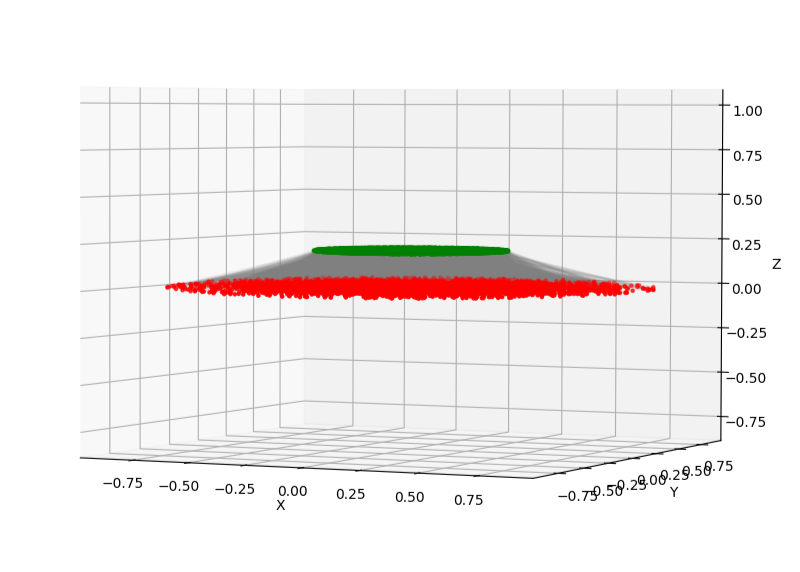
\includegraphics[width=0.49\textwidth]{images/accettanza/example4.1.png}
            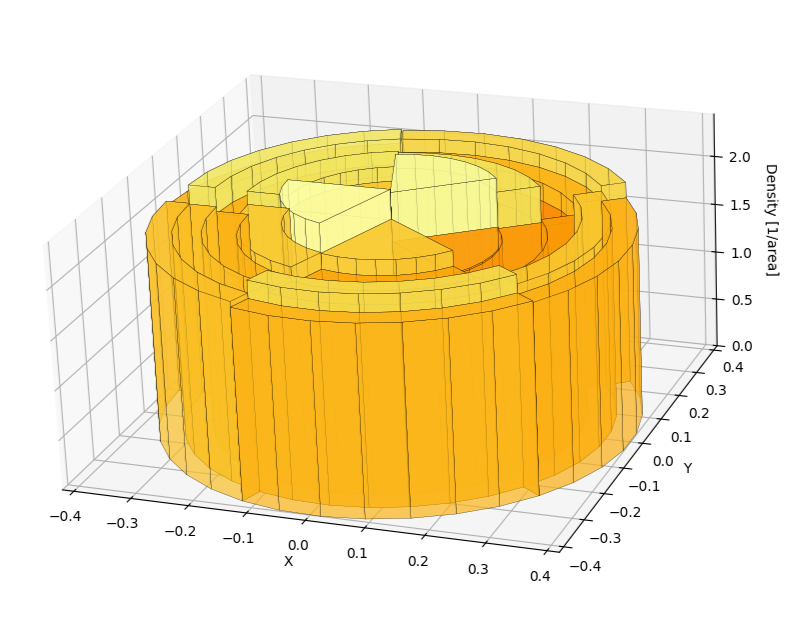
\includegraphics[width=0.49\textwidth]{images/accettanza/example4.2.png}
            \caption{Ponendo un rivelatore piccolo molto vicino alla sorgente la distribuzione appare in prima approssimazione uniforme.}
        \end{figure}

        
        \appendix
        \chapter{Codice per Arduino}\label{app:ard}
    Riporto in questa appendice il codice utilizzato per l'esperienza descritta al Capitolo \Sref{ch:ard}.
    \lstinputlisting[language=C++]{code/arduino-temp.txt}

    \backmatter
        \printbibliography  
       
\end{document}